% =====================================================================
%  Chapter 28 — The Risk Governor
% =====================================================================

\chapter{The Risk Governor}\idx{Governor}
\label{ch:governor}

The risk governor is the layer that does the work. Part VI will show that
the model's contribution to the return is approximately zero and that the
governor's contribution is positive, and that the governor is what reduces
the maximum drawdown. This chapter explains how it works and why it is
built the way it is.

\section{Two mechanisms, two purposes}

The governor has two parts, and they act on different things.

The \textbf{volatility scaler} reduces the portfolio's exposure\idx{Exposure} when the
recent realised volatility is high and restores it when it is low. It acts
on the \emph{level} of risk.

The \textbf{drawdown brake\idx{Drawdown brake}} reduces the portfolio's exposure when the
portfolio is in a drawdown, at two thresholds. It acts on the
\emph{history} of the portfolio.

The two are separate because they answer different questions, and because
they have different failure modes. The volatility scaler fails by
reducing exposure after a large move --- selling low --- and the drawdown
brake fails by reducing exposure after a sustained loss, which is
sometimes exactly what should be done and sometimes exactly wrong.

\section{The volatility scaler}

Let \(\hat{\sigma}\) be the portfolio's annualised realised volatility
over the trailing window, and \(\sigma^{*}\) the target. The scaler
multiplies every risky weight by
\begin{equation}
s = \min\left(1,\ \left(\frac{\sigma^{*}}{\hat{\sigma}}\right)^{\delta}\right),
\end{equation}
where \(\delta\) is the damping\idx{Damping} parameter and the book uses \(\delta = 0.5\).

This is volatility scaling\idx{Volatility scaling}, and it is the first of the two mechanisms this
chapter introduces. It changes the size of the position, not its sign, and
it is the layer that turns a forecast into a number of dollars.

Two details are deliberate.

The \textbf{one-sided cap}: the scaler never increases exposure. It can
only reduce it. A rule that scales up after a quiet period would be
leveraging into a calm, which is the opposite of what a protection layer
should do, and it would raise the portfolio's volatility precisely when
the drawdown brake was about to be triggered.

The \textbf{damping}: the exponent \(\delta = 0.5\) means the scaler
responds to the square root of the ratio. A volatility that doubles
reduces exposure by a factor of \(\sqrt{2}$, not by a factor of two. The
damping is what keeps the governor from becoming a feedback oscillator:
an undamped scaler would cut exposure after a volatility spike, which
would itself lower the volatility, which would restore the exposure, and
the portfolio would oscillate.

\begin{figure}[!htbp]
\centering
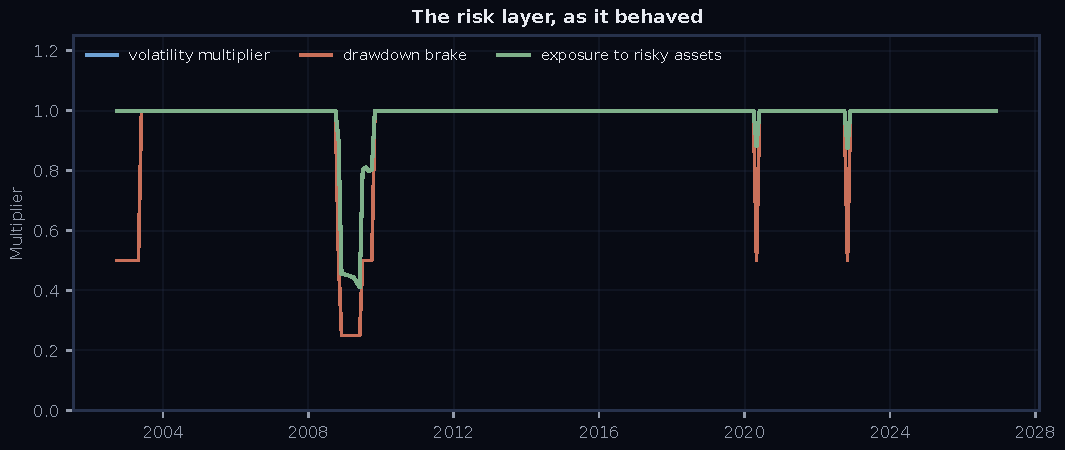
\includegraphics[width=\textwidth]{../figures/fig_governor.pdf}
\caption{The governor in operation: the portfolio's realised volatility
against its target, the exposure scale the governor applied, and the
drawdown that triggered the brake. The scaler acts on volatility and the
brake acts on the portfolio's own history, and they are visible as two
separate traces.}
\label{fig:governor}
\end{figure}

\section{The drawdown brake}

The brake is a two-level threshold rule on the portfolio's own trailing
drawdown.

Let \(d_t\) be the portfolio's drawdown at the end of month \(t\): the
fall from its running peak. The book uses thresholds of fifteen per cent
and twenty-five per cent. When the drawdown is beyond the first
threshold, the portfolio's risky exposure is cut to fifty per cent;
beyond the second, to twenty-five per cent. The remainder goes to cash.

Three design decisions are worth stating.

\textbf{The brake acts on exposure, not on orders.} It does not sell the
losing positions; it reduces what the portfolio holds and stops adding
risk. A stop-loss sells, and selling crystallises the loss and prevents
the recovery. Cutting exposure preserves the position and therefore
preserves the recovery --- and it is the behaviour Chapter 8 argued for,
because it gives the investor a reason not to override the system during
the drawdown.

\textbf{The brake is one-way within a drawdown and resets at the peak.}
Once the portfolio makes a new high, the brake releases in full. The
book does not implement a hysteretic ramp, and it says so: a more
sophisticated brake would be a hyperparameter to be tuned, and the book's
position is that a threshold rule with two stated thresholds is more
defensible than a tuned one.

\textbf{The brake is in the trial family.} Two alternative volatility
targets are run, and the drawdown thresholds are fixed rather than tuned,
but the whole governor can be turned off --- and that ablation is one of
the most informative members of the family, because it isolates exactly
what the governor contributes.

\section{What the literature says about this, and what it does not}

The governor is a volatility-managed portfolio in the sense of Moreira and
Muir, and the book must deal with the fact that the most careful
replication of that result found it does not work.

Moreira and Muir's 2017 result in the \emph{Journal of Finance} is
striking: scaling exposure inversely to the past variance of the
portfolio's excess return raised the Sharpe ratio of a market-timing
strategy from 0.78 to 1.41 over their sample. Cederburg, O'Doherty, Wang
and Yan's 2020 replication in the \emph{Journal of Financial Economics}
examined 103 equity strategies and found that the volatility-managed
versions \emph{do not} systematically outperform, that the real-time
versions earn lower compound returns and lower Sharpe ratios than the
realised ones, and that the failure comes from the structural
instability of the regressions the method requires.

The book takes the replication's finding seriously and does not claim
that the governor will raise a Sharpe ratio. What it claims is narrower
and is supported by the book's own measurement: the governor reduces the
depth and the duration of the worst episode, at a stated cost in compound
return, and it does so with a mechanism that does not depend on a
forecast being right.

\begin{takeaway}[The distinction]
The governor does not predict. It responds to the portfolio's own realised
volatility and its own realised drawdown, both of which are known at the
time. A mechanism that requires no forecast cannot be wrong about the
future, and therefore cannot fail in the way a forecast-based mechanism
fails.
\end{takeaway}

\begin{keytakeaways}
\item Two mechanisms: a one-sided, damped volatility scaler acting on the
level of risk, and a two-level drawdown brake acting on the portfolio's
history.
\item The scaler never increases exposure and responds to the square root
of the volatility ratio, which is what stops it oscillating.
\item The brake cuts exposure rather than selling positions, which
preserves the recovery and gives the investor a reason not to override
the system.
\item Moreira and Muir's result does not replicate, and the book claims
only what it measures: a shallower and shorter worst episode, at a
stated price, from a mechanism that requires no forecast.
\end{keytakeaways}
